\chapter{Estuaries}
\label{chap:Estuaries}

\includegraphics[width=6.5in]{figs/ed_mcnichol_boundary_smaller.jpg}


\Wikiref{Estuaries} are semi-enclosed basins of water that are strongly influenced by freshwater sources (i.e. a river) or evaporation, yet have an opening to the open ocean where salty water can get into the basin.  The semi-enclosed nature of the basin allows time for mixing between the fresh and the ocean water, and the density differences created drive a strong \emph{overturning circulation} in the basin, such that much more water is drawn up the estuary than starts out flowing in from the river.  Here we attempt to describe how this circulation works. How estuarine circulation occurs is subtle, but not terribly difficult to qualitatively.  It is, however, not amenable to simple mathematical description, which may explain its omission from basic texts.

It is a little unusual to start a course with something as dynamic as an estuary. We do this as a bit of foreshadowing for the rest of the course, and because Saanich Inlet is an estuary, and we will be considering Saanich Inlet in the context of the course project.  

\section{Pressure differences}

Before we start, it is helpful to think about how pressure differences drive flows.  A fluid moves due to friction (i.e. the wind blowing over the surface), direct action (i.e. a paddle pushing water), or pressure forces.  Pressure forces are unique to fluids, and are the forces that the water can exert on itself. In general they tend to move water so that pressure differences are evened out, i.e. the water pushes itself from high pressure regions to low pressure regions.  
\begin{marginfigure}
  \centering
  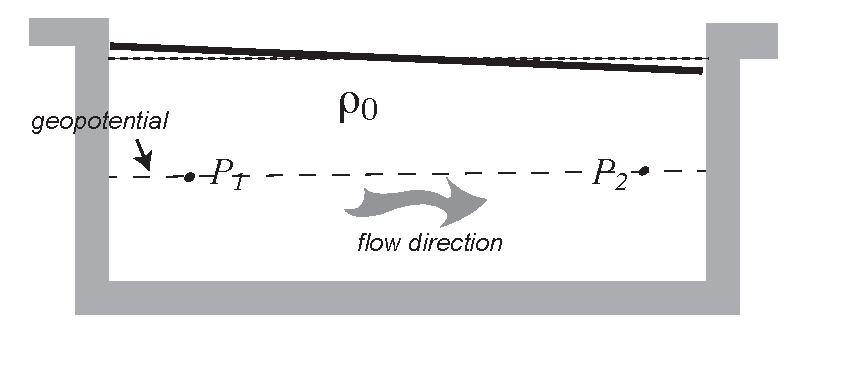
\includegraphics[width=3in]{figs/PdiffSurf}
  \caption{A body of water of uniform density with a tilted upper
    surface.  Note that P1 and P2 are at the same geopotential height (i.e. their value of z is constant)}
  \label{fig:PdiffSurf}
\end{marginfigure}
 
If the sea-surface is tilted, then the pressure will be greater where the sea surface is high than where it is low; in \fref{fig:PdiffSurf}, $P_1>P_2$.  This will drive the flow from left to right.  \emph{Note} pressure increases with depth, so when we think about how the pressure moves water, we need to think about the pressure along a ``geopotential'' surface (ie. a surface along which the water would be flat).  For our purposes, this is a set distance below the flat surface of the water.


In general, it is a good rule to think that the water will move in the direction that will lead to a flattening of the surface.  The resting state of the body of water is to have a flat surface, as indicated with the dashed line at the surface in \fref{fig:PdiffSurf}.  

The situation is more complicated if we add density variations. Consider just tipping the interface of a two-layer fluid (\fref{fig:PdiffTiltInt}). (This is actually hard to do, but just
 imagine).  At first, the pressure difference in the upper layer is zero ($P_3=P_4$) because the upper interface is not tilted.  However, there is more dense water on the left side than the right, so there is a pressure gradient below the interface, $P_1>P_2$, driving deep water to the right.

\begin{marginfigure}
  \centering
  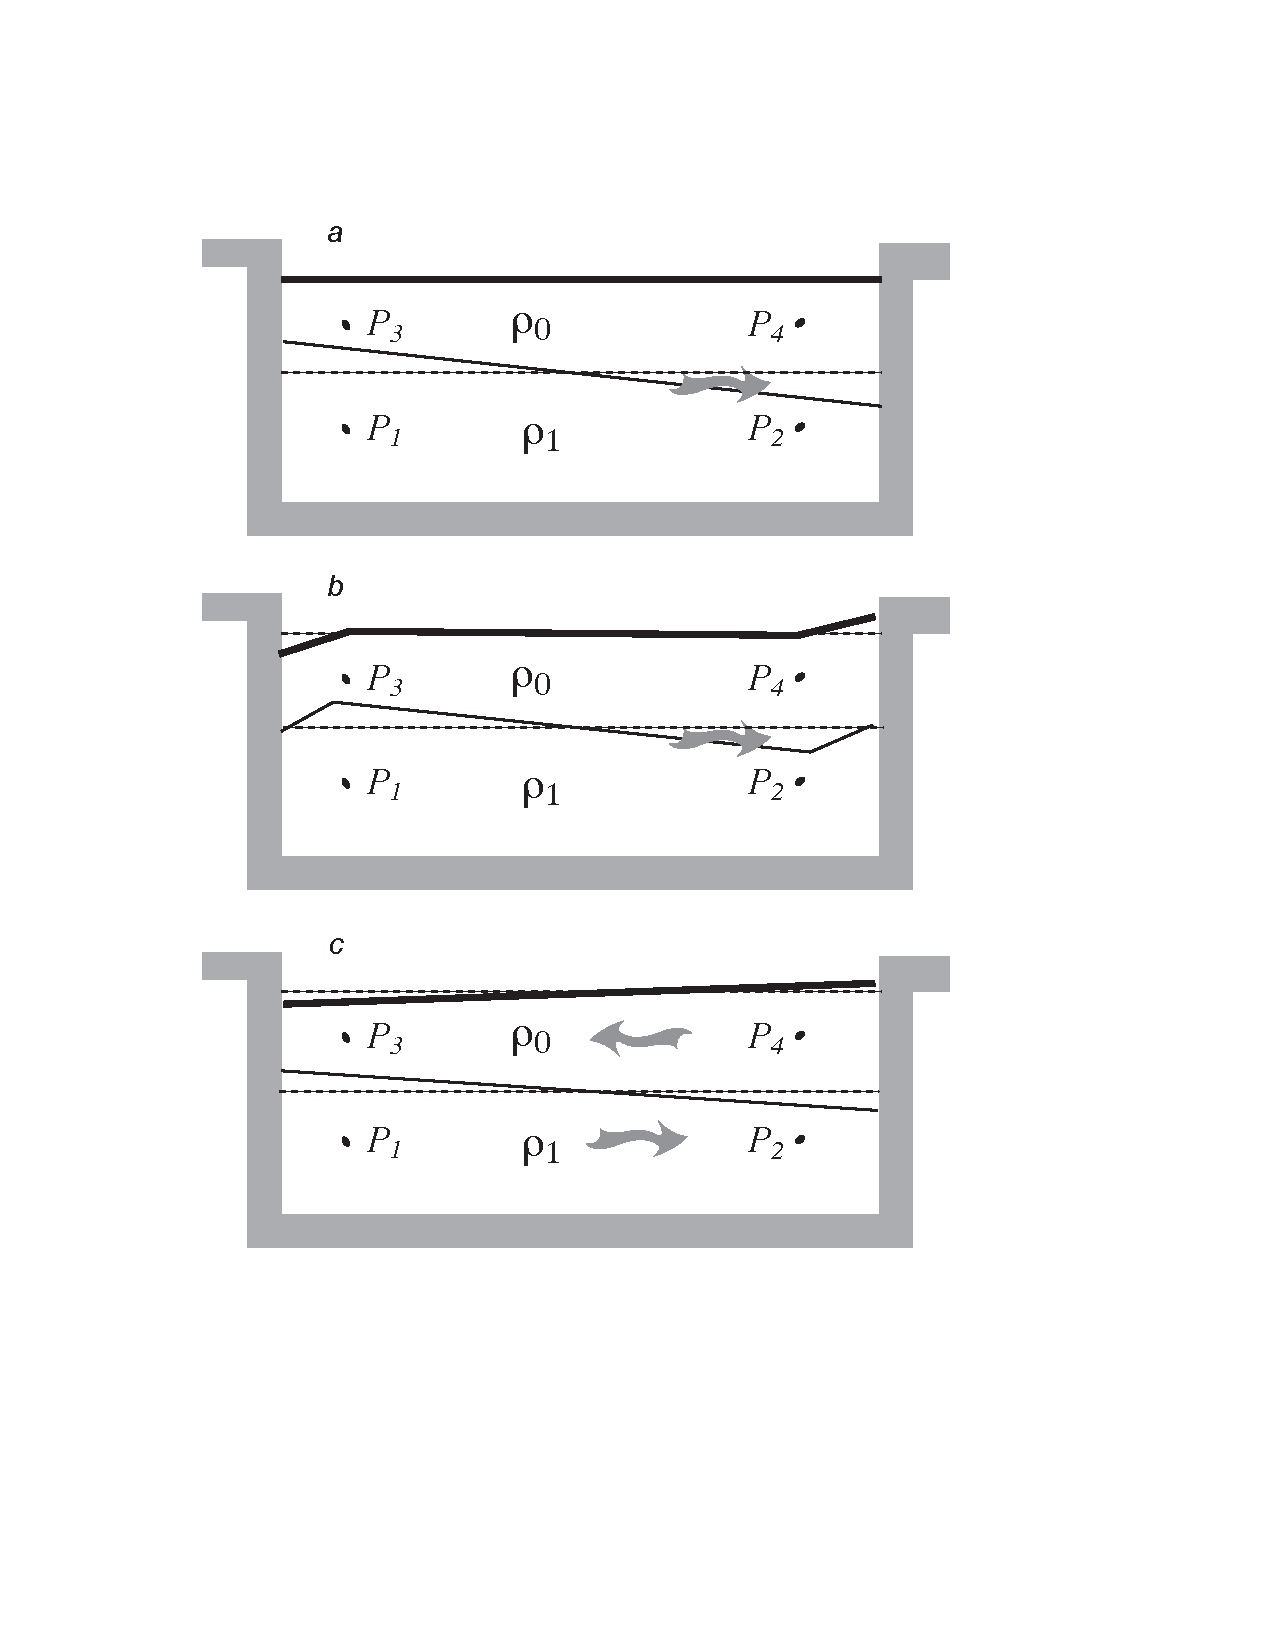
\includegraphics[width=3in]{figs/PdiffTiltInt}
  \caption{A two-layer body water with an interface that is initially
    tilted. See text for the description. }
  \label{fig:PdiffTiltInt}
\end{marginfigure}


This leads to more water, in total, on the right hand side than the left side (\fref{fig:PdiffTiltInt}b).  This makes a surface pressure gradient that tends to drive the upper layer to the left ($P_4>P_3$). This surface pressure gradient is set up \emph{very} quickly, and only involves a tiny amount of water in order to drive the surface-layer flow to the left.

The water column will slosh around for a while, but friction will eventually damp the motions and the interfaces will be flattened as indicated with the dashed lines (\fref{fig:PdiffTiltInt}c).

\begin{marginfigure}
  \centering
  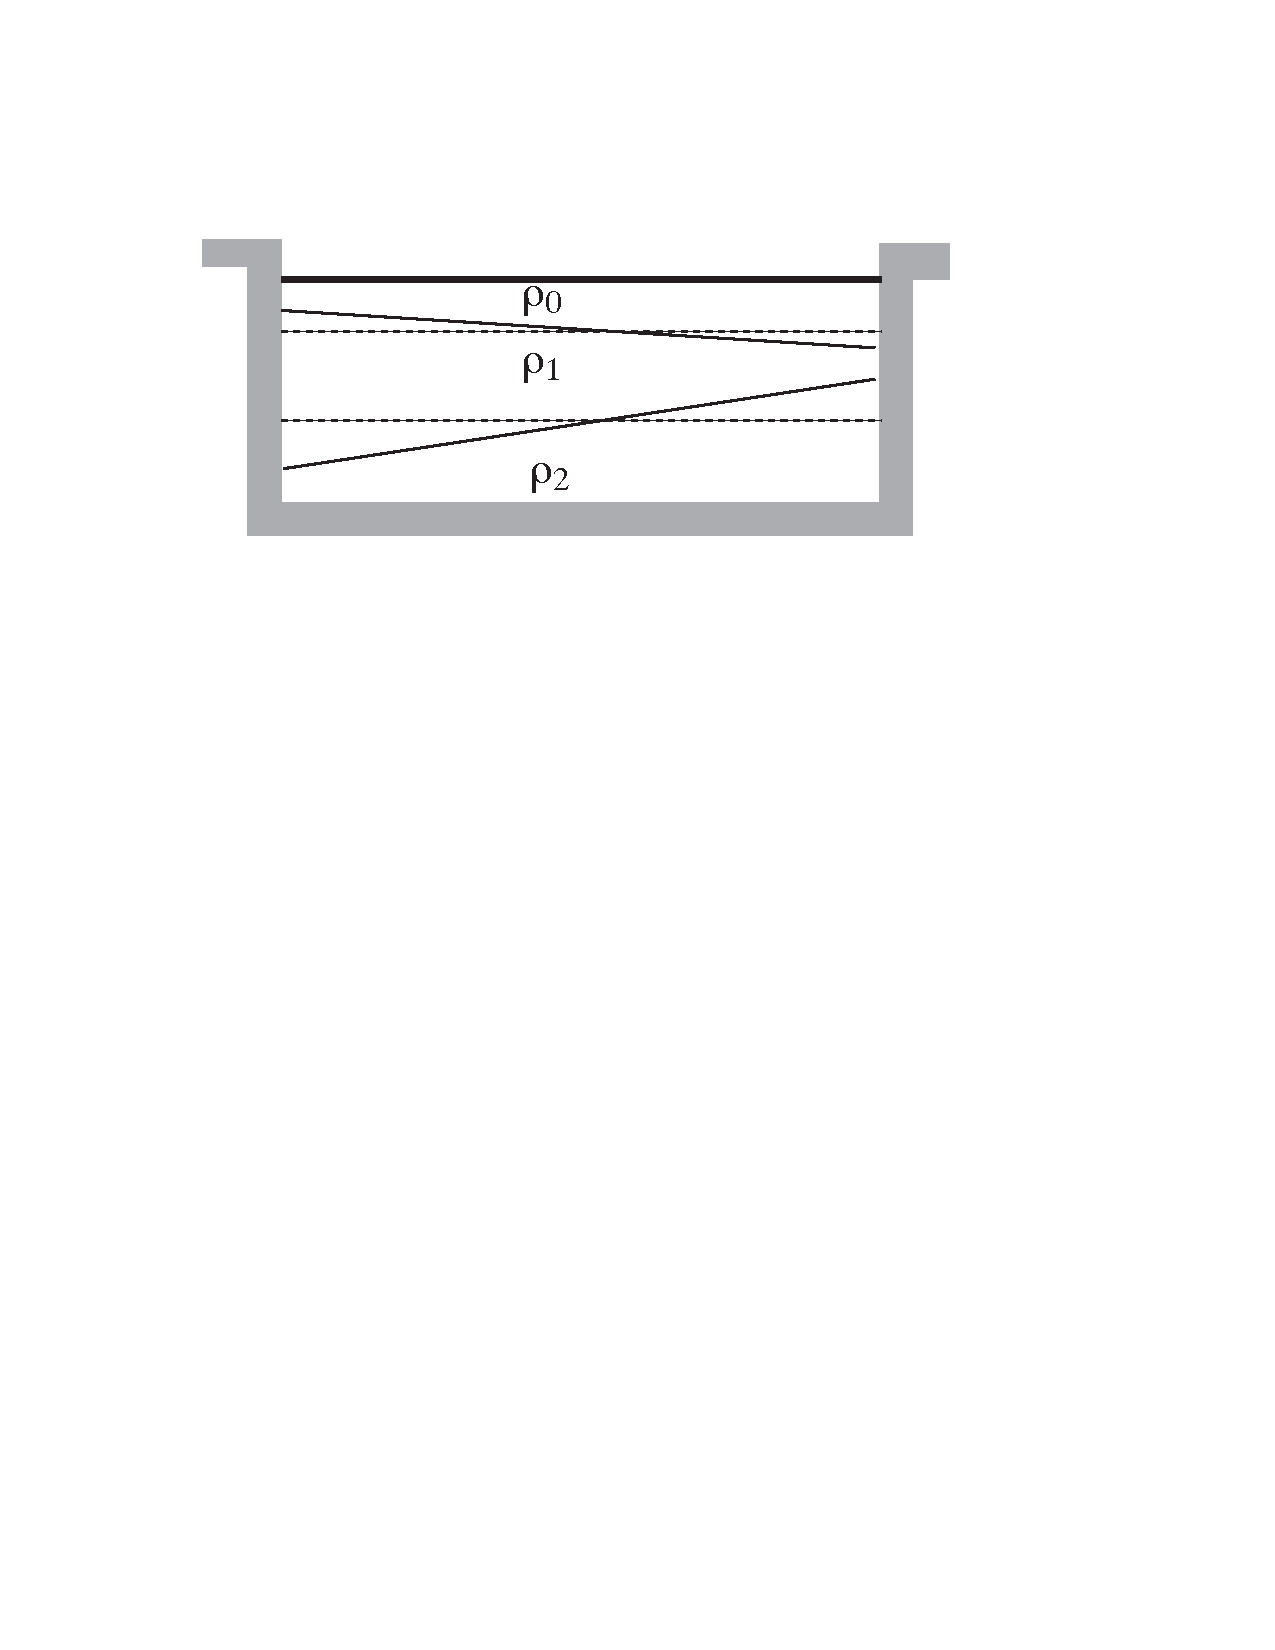
\includegraphics[width=3in]{figs/PdiffTilt3Int}
  \caption{A three-layer body water with tilted interfaces. }
  \label{fig:PdiffTilt3Int}
\end{marginfigure}

Again, the general idea is that the body of water has pressure gradients in it that drive a flow that will tend to flatten the layers.

\studyq{In \fref{fig:PdiffTilt3Int}, what direction does each layer flow?}

\studyq{If the density differences between the layers are equal, which layer will initially have the strongest flow?}


\section{Estuarine Flow}

\subsection{Salt-wedge estuary}

\emph{Estuaries} are bodies of water with opposing buoyancy sources at their ends, usually a river at the head and the ocean at the mouth.  The buoyancy difference usually arise from the salt content of the water, with fresh water being ``lighter'', or more buoyant, than salty water.   The simplest situation is a river spills into the ocean, spreads out and becomes a buoyant plume (\fref{fig:EstuaryNoMix}).  If we quantify the river volume transport as $R$ (typically in units of $m^3\,s^{-1}$) then in \Wikiref{steady state} the transport out the mouth of the estuary will be $Q_o=R$.  The deep ocean layer will be stagnant.

\begin{figure}[htb]
  \centering
  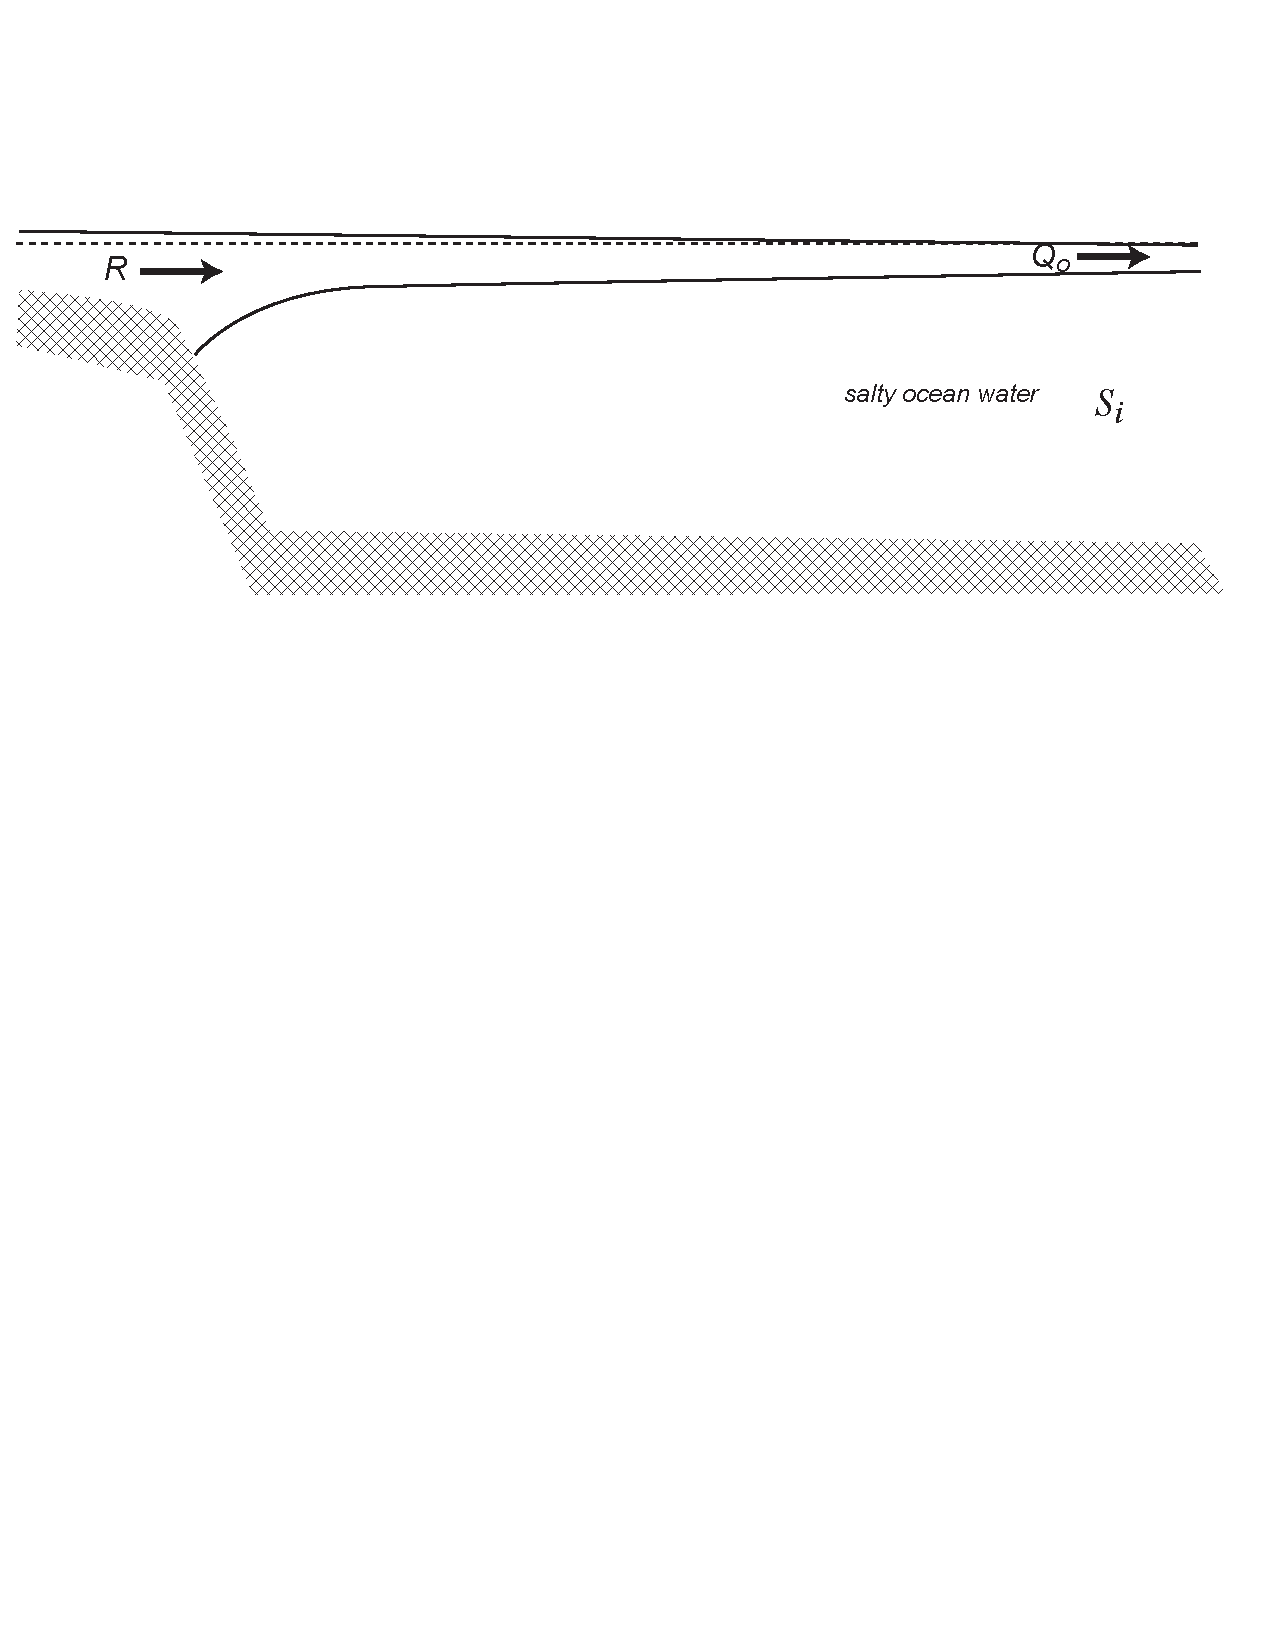
\includegraphics[width=3.5in]{figs/EstuaryNoMix}
  \caption{A salt-wedge estuary and river plume.  The river discharges
    into the salt water without substantial mixing.}
  \label{fig:EstuaryNoMix}
\end{figure}

This type of estuary is called a \emph{salt-wedge estuary}.  The mouth of the Fraser River is a classic example of a salt-wedge estuary with a spreading plume (\fref{fig:GeyerFarmerFig3}).  Fresh water runs over salty with a small amount of mixing between the two layers.  The salinity goes from 2 psu to 24 psu (1 psu $\approx$ 1 part-per-thousand, or gram of salt per kilogram of water) in just a few meters vertically. This sharp front moves back and forth with the tide, a typical feature of most salt-wedge estuaries.

\begin{figure}[htb]
  \centering
  \includegraphics[width=4in]{figs/GeyerFarmerFig3}
  \caption{Salinity contours in mouth of the Fraser River. Salinity has units of parts per thousand, or ppt.  So 1 ppt means 1 gram of salt per kilogram of water. The unit ``psu'' is also often used, meaning practical salinity unit, with $1\ \mathrm{psu}=1\ \mathrm{ppt}$.  The river
    is on the left, the ocean on the right. \citep{geyerfarmer89} }
  \label{fig:GeyerFarmerFig3}
\end{figure}

\subsection{Fjord-type estuary}

Unlike a \emph{salt-wedge} estuary, most estuaries have an ``exchange flow'' that is much stronger than  the river flow.  This flow is driven by vertical mixing that in turn creates tilted ``isopycnals'', or constant density surfaces.  These tilted isopycnals want to slump due to the pressure gradients that are set up, as discussed above.

As an example, imagine the situation pictured in \fref{fig:EstuaryLocal}.  Here a river flows into salty water.  If turbulent mixing is driven by strong tidal flow over the topographic bump in the middle of the estuary, then intermediate-salinity water will be formed.  This intermediate-salinity water will be denser than the river water, but lighter than the ocean water, and will set up a flow that is pictured in \fref{fig:EstuaryLocal}b.

\begin{figure}[htb]
  \centering
  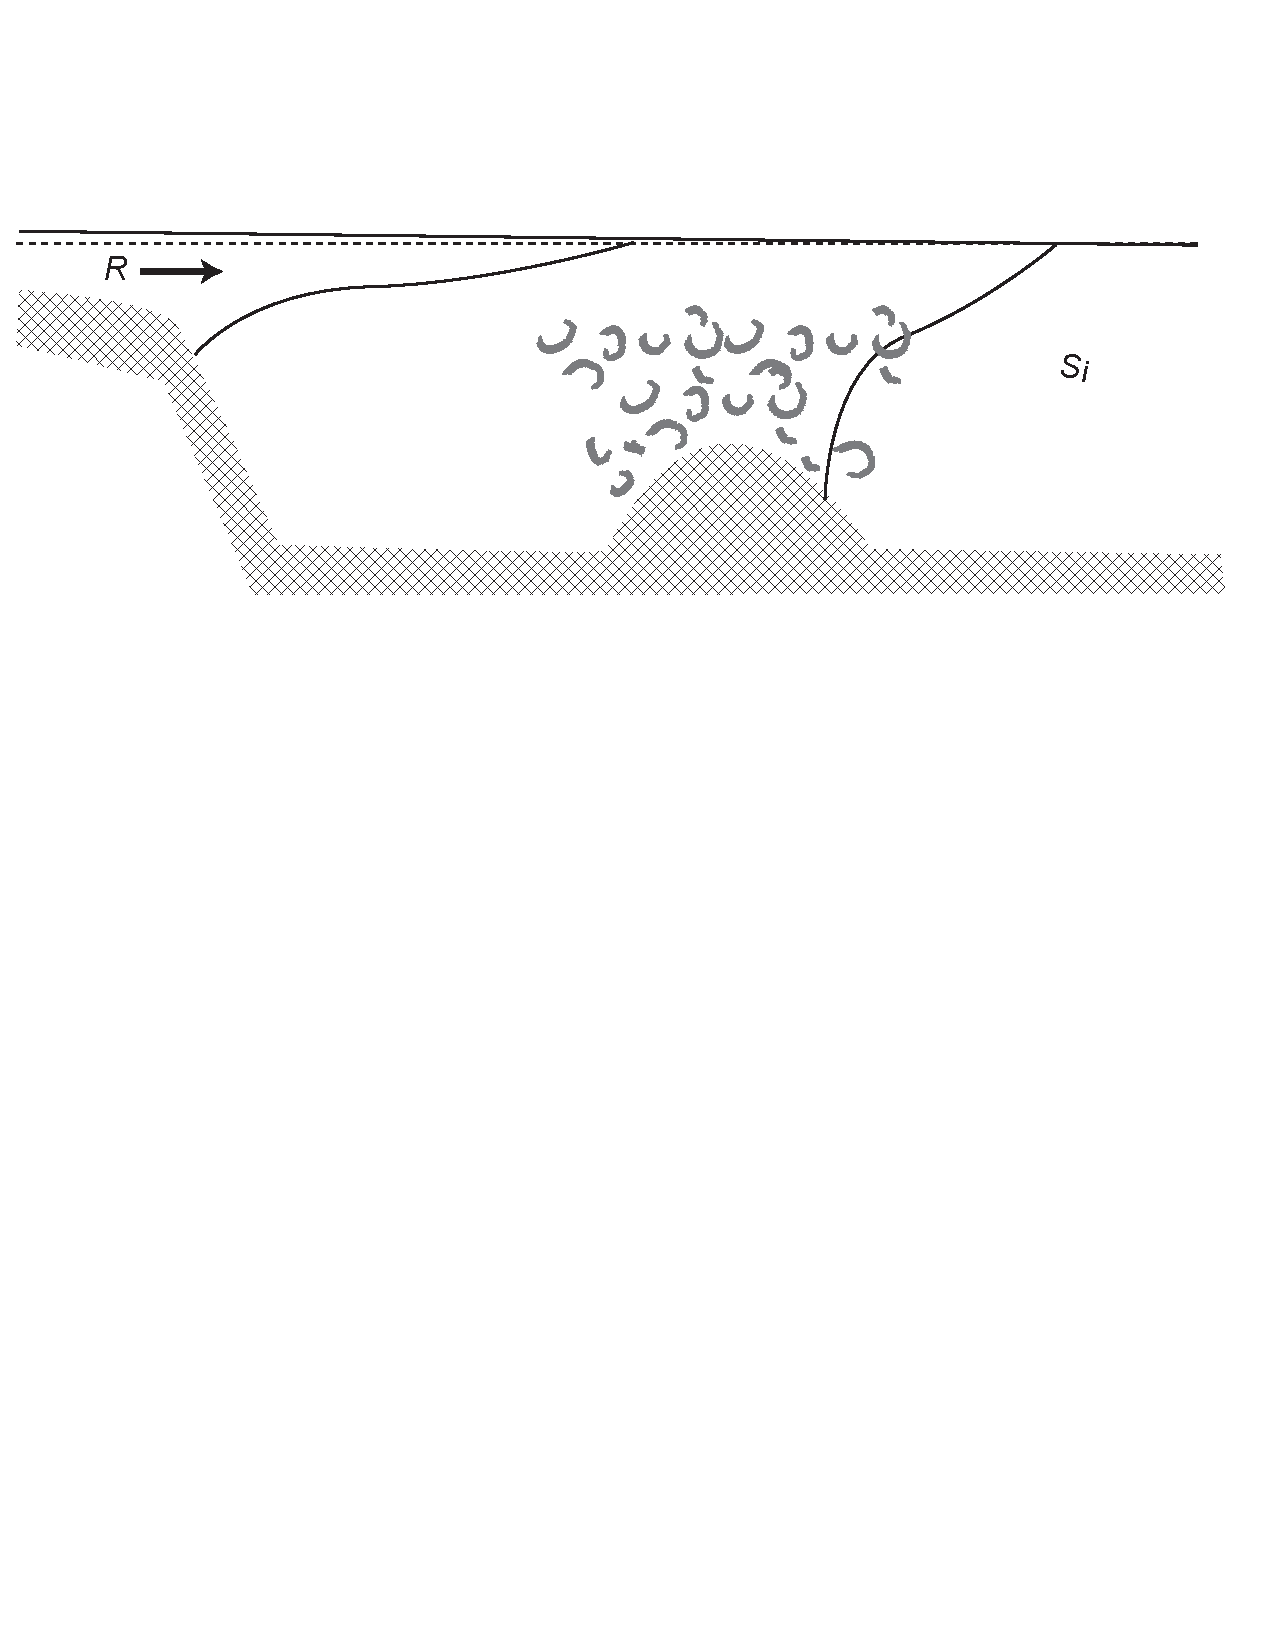
\includegraphics[width=3.5in]{figs/EstuaryLocal}
  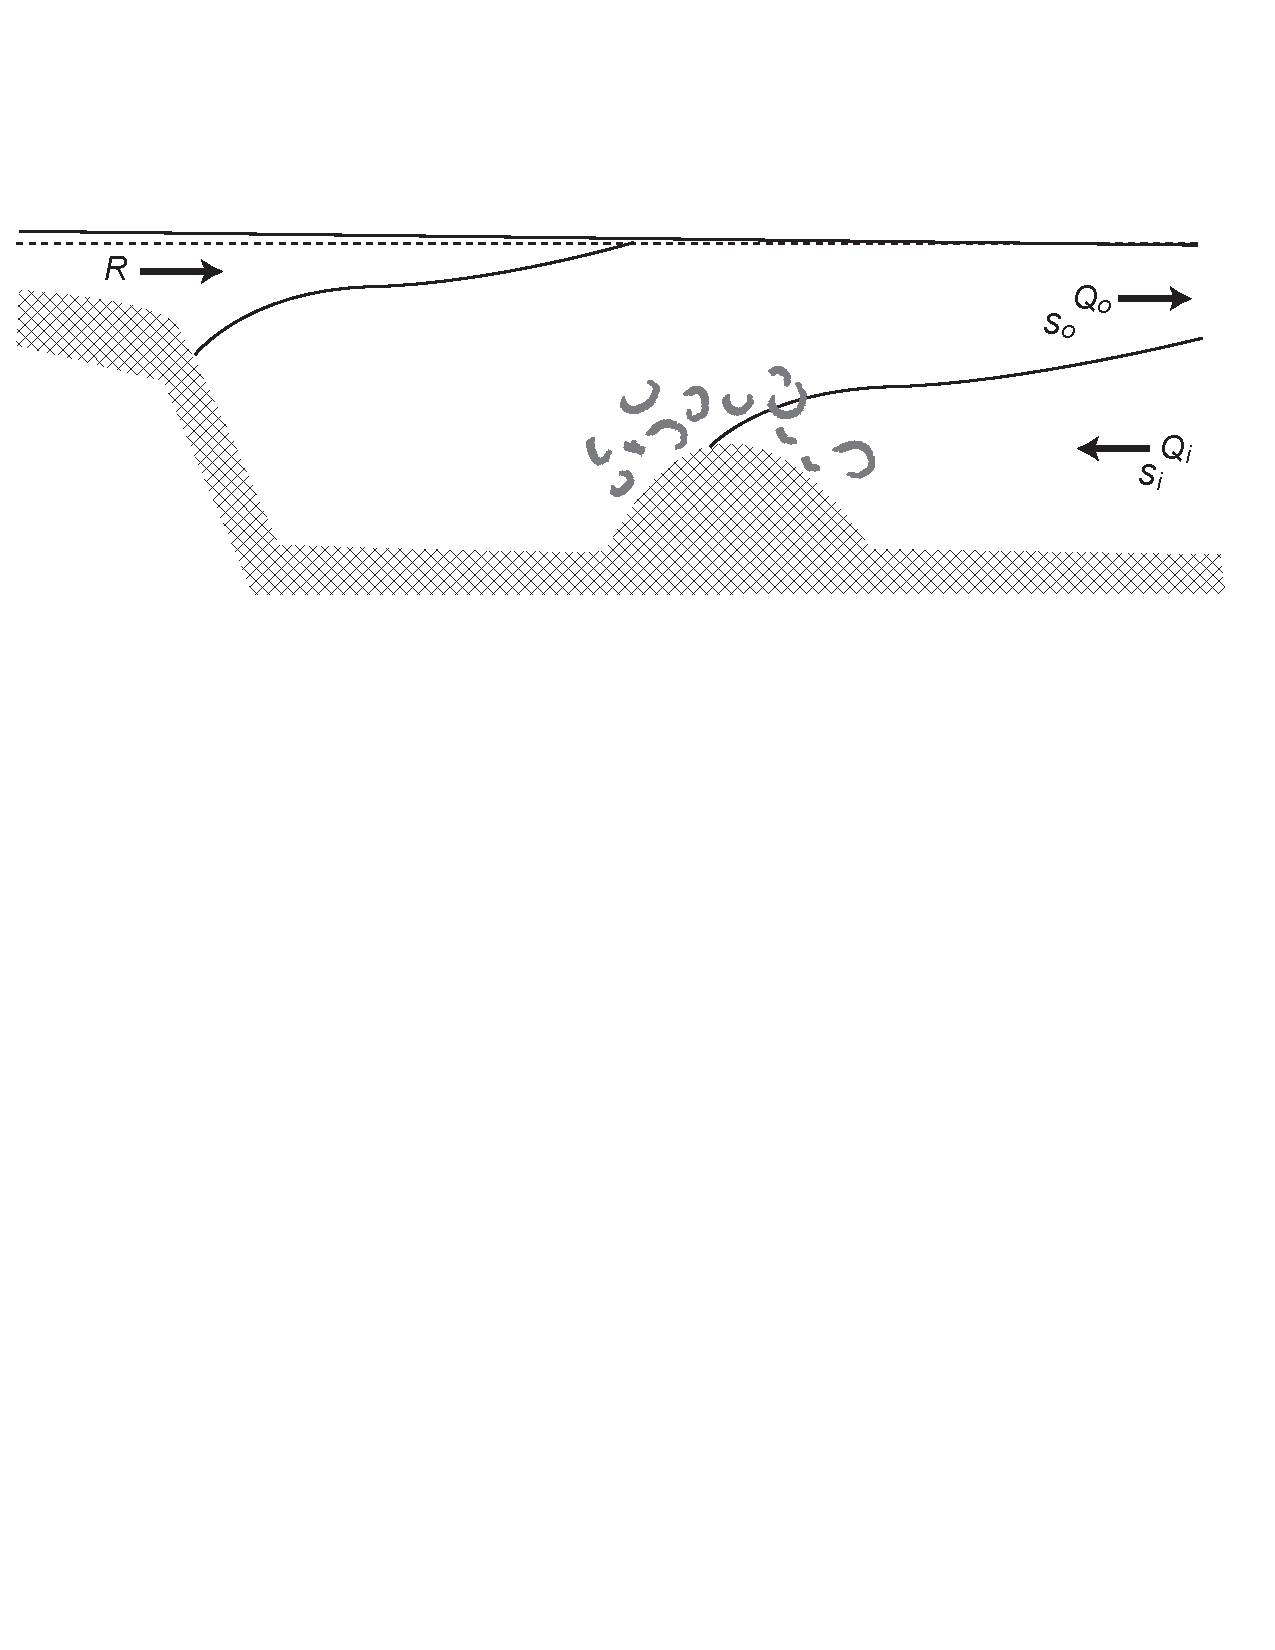
\includegraphics[width=3.5in]{figs/EstuaryLow}
  \caption{The effect of weak local mixing on flow in a fjord-type
    estuary. Intermediate salinity water is formed by the mixing which
  drives a flow out to sea.  In this figure, ``isohalines'' are indicated by the contours (constant salinity surfaces) and will correspond to ``isopycnals'' (constant density surfaces) in most cases.  }
  \label{fig:EstuaryLocal}
\end{figure}

Determining the steady-state for such a flow is not trivial, and not very conducive to theoretical formulation.  However, general tendencies can be determined.  If there is more mixing, more intermediate water is formed. In steady state, this intermediate water must be flushed away, so there is a stronger circulation.  Conversely, if the mixing is weaker, less intermediate water is produced, weakening the circulation.

\subsection{Flood-plain estuaries}

The more mixing that takes place, the more vertical the isopycnals, and the stronger the exchange flow that is driven (relative to the river flow).  The salt and density fields also become much more complicated.  In shallow estuaries, of which the Chesapeake Bay is an excellent example, mixing from bottom stress and the winds tends to affect the whole water column, not just near topographic features.  This sets up large along-estuary salinity and density gradients (\fref{fig:EstuaryHigh}). These types of estuaries tend to have much stronger amplification of the river flow ($R$) because of the extra mixing.

\begin{figure}[htb]
  \centering
  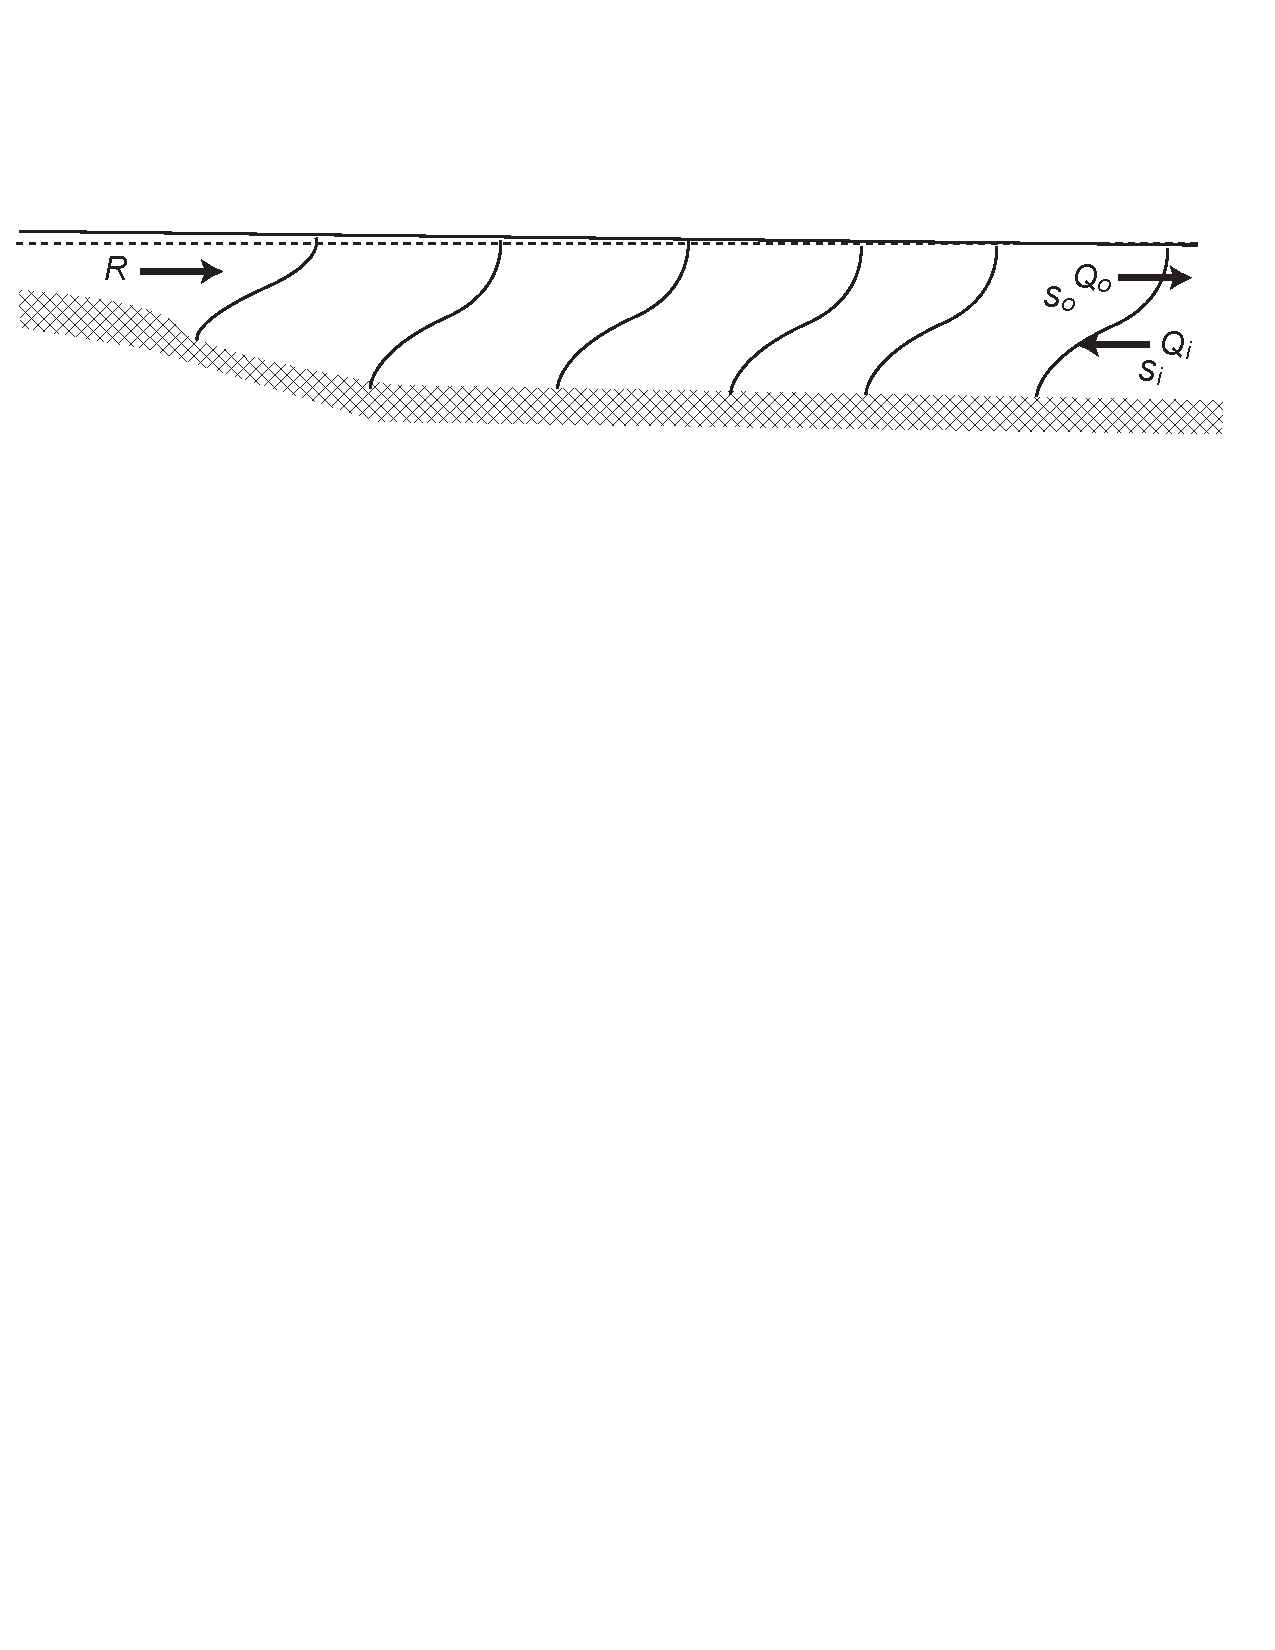
\includegraphics[width=4in]{figs/EstuaryHigh}
  \caption{A flood-plain estuary schematic.  Salinity increases from
    the head to the mouth, with weak vertical gradients.  }
  \label{fig:EstuaryHigh}
\end{figure}


An example from an arm of the Chesapeake demonstrates how such an estuary may look (\fref{fig:Elliott76Fig8}).  Up estuary  of Maryland Point, the estuary is really a river with no salinity.  However, unlike the salt-wedge estuary, there is a gradual horizontal gradient of many kilometers before salty water is found.  Note that even at this point the water is still only 12 psu, and that the Chesapeake Estuary continues for hundreds more kilometers before open-ocean water is found.

\begin{figure}[htb]
  \centering
  \includegraphics[width=4in]{figs/Elliott76Fig8}
  \caption{A salinity cross-section from the Upper Potomac estuary,
    part of the Chesapeake Bay estuarine system \citep{elliott76}.}
  \label{fig:Elliott76Fig8}
\end{figure}

The whole estuary has been measured and simulated numerous times.  A recent example is shown in \fref{fig:LiEtAl05Fig5}.  Here the upper layer of fresher water can be seen flowing south and seaward.  There is a strong return flow in the bottom 20 m.  Note that the volume transport of the return flow is not accurately represented by these velocities, since they do not take into account the fact that the Bay widens considerably as it travels further south.
\begin{figure}[htb]
  \centering
  \includegraphics[width=3in]{figs/LiEtAl05Fig5}
  \caption{A salinity and mean velocity sections from a numerical
    model of the whole Chesapeake Bay \citep{lietal05}}
  \label{fig:LiEtAl05Fig5}
\end{figure}

Also note the lenses of fresher water that appear along the estuary. These occur because of rivers along the length of the estuary. This complicates the simple picture given above, but the general trend of the flow remains unchanged.



\subsection{Time-dependence}

Time dependence changes the steady-state balance in estuaries in three main ways.  First, the fresh-water input at the head of the estuary can change (\fref{fig:SchubelPritchard86}).  This significantly changes the salinity content of the estuary and the estuarine circulation.  Somewhat paradoxically, the increased river flow can lead to a decreased estuarine flow.  For instance in the Apr 1968 panel the isopycnals are much less tilted than in the Oct panel, indicating enhanced flow.  The balance here, however, is not a perfect one, and determining the exact response if the river forcing changes depends on the mixing response.  Strong vertical density gradients caused by fresh water influx can suppress turbulence and hence reduce the mixing required to drive the exchange flow.

\begin{figure}[htb]
  \centering
  \includegraphics[width=4in]{figs/SchubelPritchard86Fig4}
  \includegraphics[width=4in]{figs/SchubelPritchard86Fig5}
  \includegraphics[width=4in]{figs/SchubelPritchard86Fig6}
  \caption{Salinity in the Chesapeake as it varies due to river
    discharge over the year (bars on left) \citep{schubelpritchard86}.}
  \label{fig:SchubelPritchard86}
\end{figure}

A second effect that can change the forcing of an estuary is that  the ocean water at the mouth of the estuary can change salinity due to seasonal changes in the open ocean.  This tends to be a smaller effect because the salinity differences, even in coastal waters, tend to be less pronounced.  However, coastal waters are subject to seasonal changes due to coastal upwelling and downwelling.  During upwelling, denser water can be found at the estuary mouth, whereas during downwelling the density can decrease.

Finally, there is a time dependence to the mixing that ultimately drives the enhanced estuarine circulation.  The most regular source of time-dependence is the tidal forcing. This varies with the fortnightly (every two weeks) modulation of the tide, and with the long-term perigree/apogee variations of the moon-earth-sun system.  More mixing during the \emph{spring} tides leads to \emph{isohalines} that are more tilted (\fref{fig:BlantonEtAl00Fig5}) which therefore drive more circulation.

\begin{figure}[htb]
  \centering
  \includegraphics[width=3in]{figs/BlantonEtAl00Fig5}
  \caption{Salinity in the Mira estuary (Portugal) during neap and spring tides
    \citep{blantonetal00}.}
  \label{fig:BlantonEtAl00Fig5}
\end{figure}

\clearpage
\subsection{Topographic blocking (mostly in fjords)}

One final topic is topographic blocking.  Fjords are often demarcated from the ocean by underwater sills (terminal moraines left over from glaciations).  These sills can be quite tall and sometimes the tides are not strong enough to bring the densest water from the ocean-side of the sill over the sill (\fref{fig:EstuaryBlocking}a).  The estuarine circulation carries on as normal above this depth, but the deep ocean layer does not make it into the landward basin.  This is called ``blocking''.

However, occasionally strong tides perhaps enhanced by atmospheric forcing will conspire to provide enough energy for the densest water to get over the sill.  This dense water will spill over the sill and, if it does not mix, will reach the bottom of the fjord (\fref{fig:EstuaryBlocking}b).  For some fjords this happens every spring-neap cycle.  For others only when the spring tide is particularly large, or the water on the seaward side denser than usual.  

\begin{figure}[htb]
  \centering
  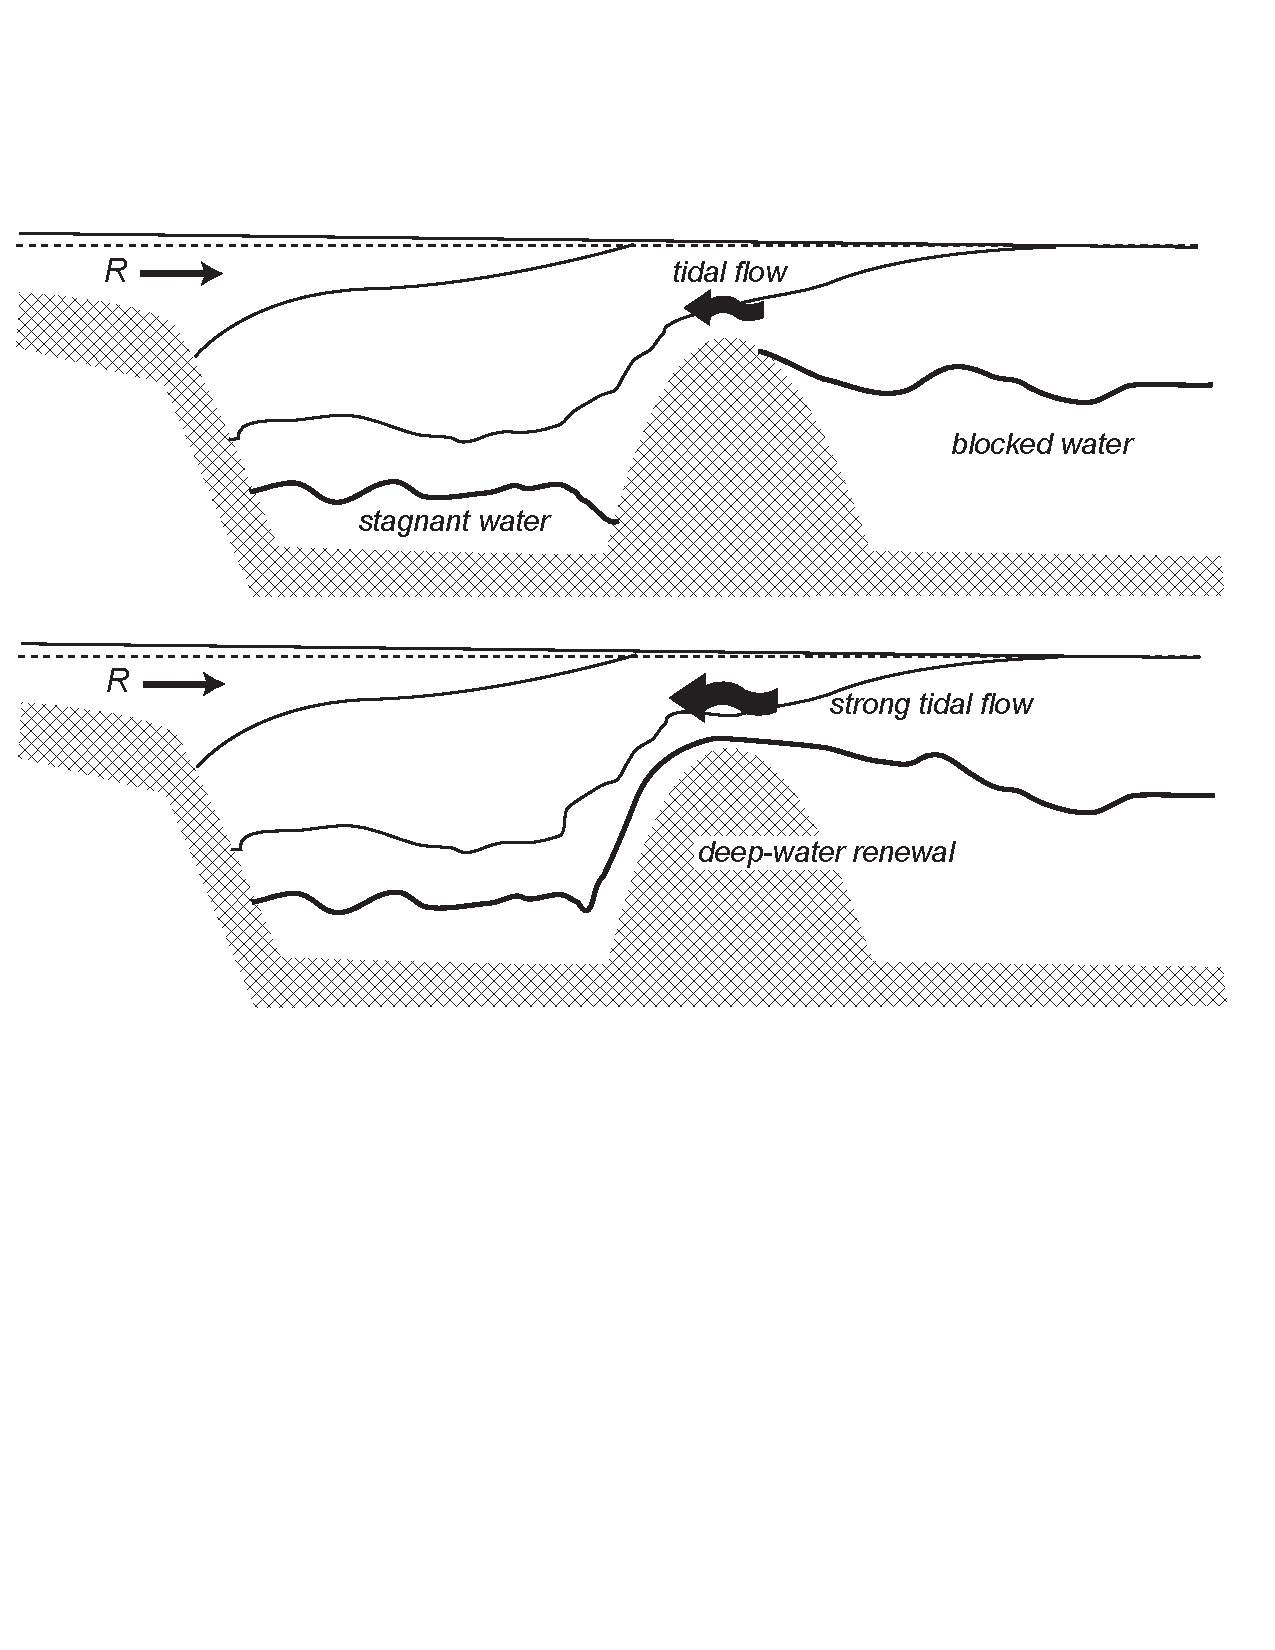
\includegraphics[width=3in]{figs/EstuaryBlocking}
  \caption{A narrow-silled fjord with blocking of deep water, and a
    deep-water renewal event.}
  \label{fig:EstuaryBlocking}
\end{figure}

Conversely, if the sill is broad, or has a lot of horizontal constrictions, deep-water renewal can happen on the exact opposite phase of the spring-neap cycle (\fref{fig:EstuaryBroadSill}).  During spring tides the incoming dense water is subjected to so much mixing that it is mixed away before it can reach the inner basin.  It is only during neap tides with enough velocity to push the dense water into the inner basin, but not so much as to cause excessive mixing that deep-water renewal can take place.

\begin{figure}[htb]
  \centering
  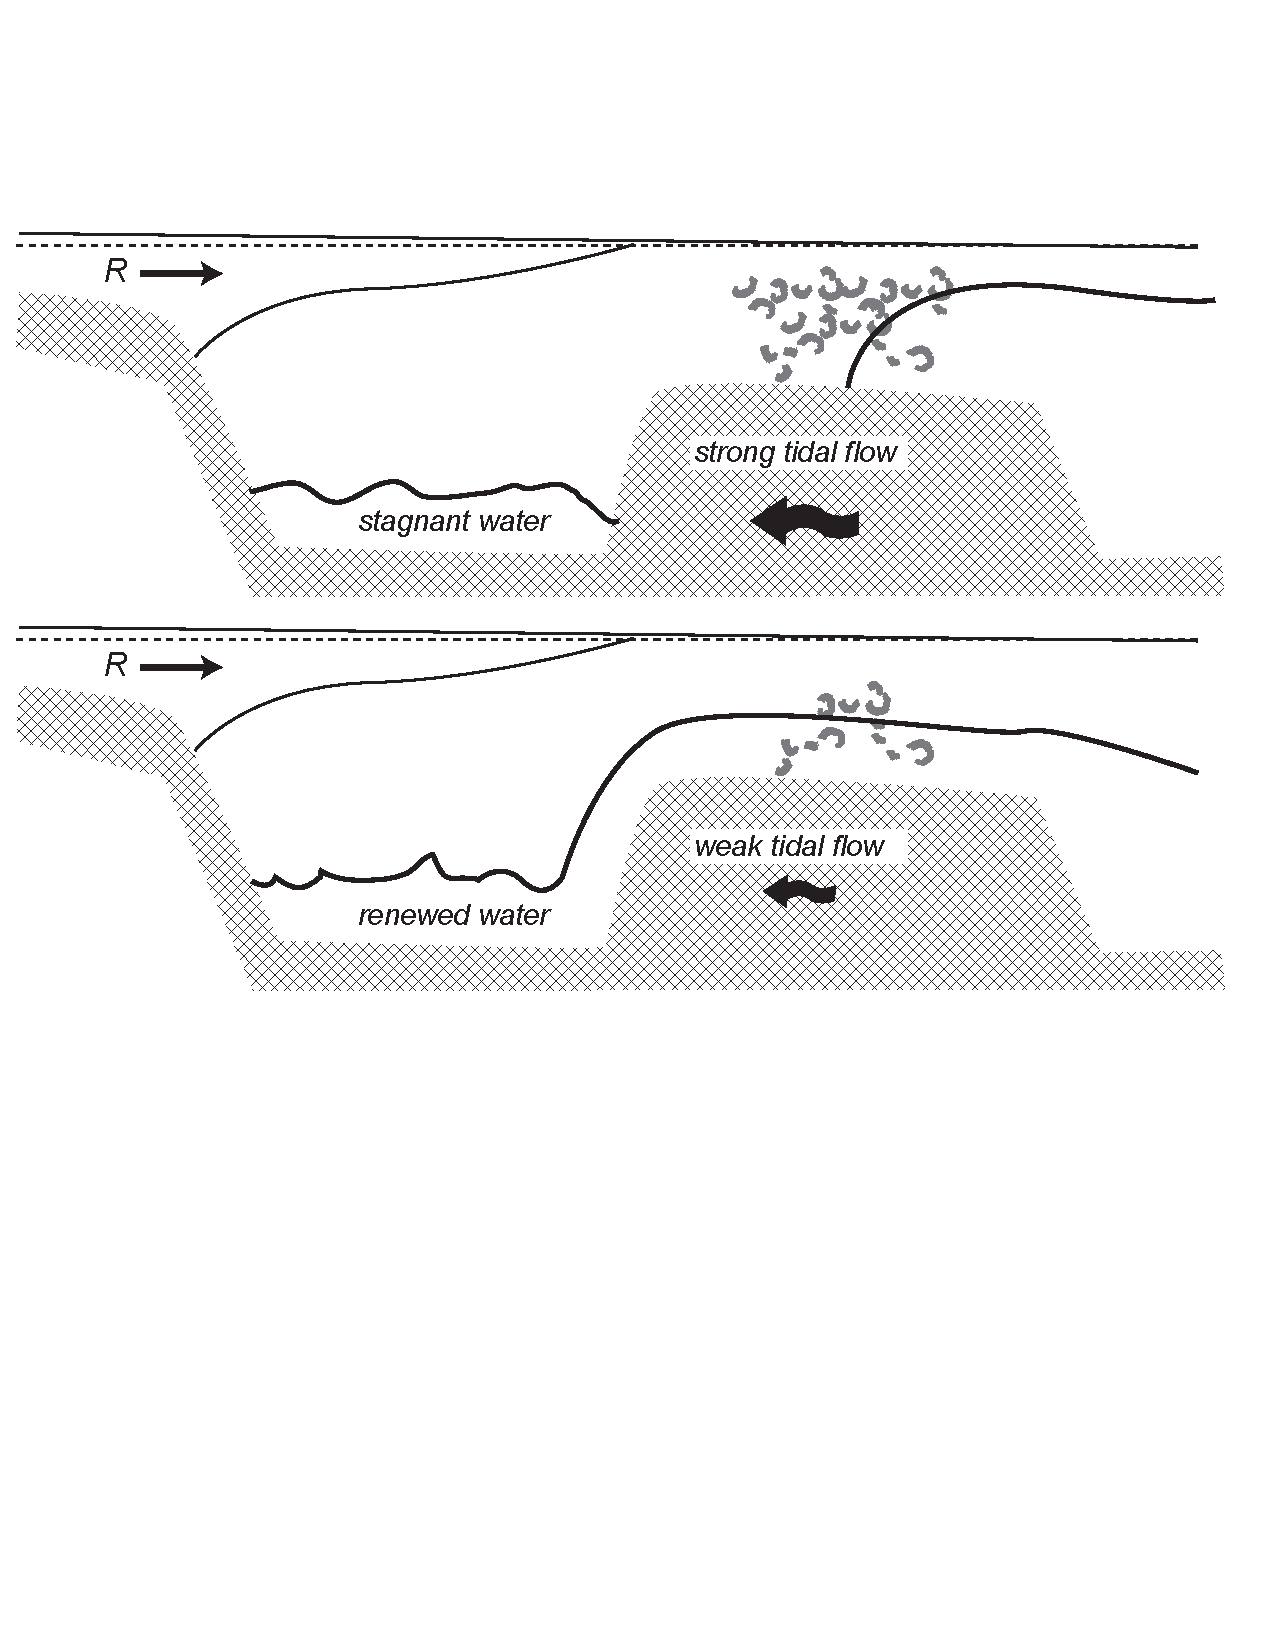
\includegraphics[width=3in]{figs/EstuaryBroadSill}
  \caption{A broad-silled fjord with blocking of deep water during
    spring tides, and a deep-water renewal during neaps.}
  \label{fig:EstuaryBroadSill}
\end{figure}



\section{Quantifying the Circulation}

See also, Open University Sec 6.2

Estuaries are a great example of mass and volume conservation. These concepts are very important for all of oceanography (and probably most of science in general).  Most people are familiar with the concepts, but laying out the mathematics takes some care (often just keeping the units straight!).

In an estuary, water flows in the river mouth, and in and out at the ocean end of the estuary.  If everything is in ``steady-state'' we can write equations that relate the incoming mass of water and mass of salt to the outgoing, and make assumptions about the flow based on those measurements.  The discussion below indicates how that is done.

\subsection{The Conservation of Volume}

Suppose we are interested in the dynamics of a body of water, say a rectangular swimming pool.  The pool has a hose pumping water into it at a rate of volume transport of $q \mathrm{[m^3s^{-1}]}$.  If its surface area  $A$, how fast is the water rising in the pool?

Here the answer is relatively easy.  The speed at which water rises in the pool is $w=q/A$, the volume transport divided by the surface area.  Here we have applied the conservation of volume:
\begin{equation}
  \label{eq:VolCons}
  \frac{\mathrm{d}V}{\mathrm{d} t} = -\sum_i q_i + \sum_j s_j.
\end{equation}
where $V$ is the volume of fluid in the body we are studying, $q_i$ are individual transports out of (positive) or into (negative) the volume.  The last term is the sum of the sources (positive) and sinks (negative) inside the volume, and is included for completeness.  For the conservation of volume of water, a sink could be evaporation, and a source rainfall.  We differentiate such source and sinks from the ``advective'' transports (caused by water velocity) because the physics is distinct.

Formally, this should really be conservation of mass in the volume. In which case:
\begin{equation}
  \frac{\mathrm{d}}{\mathrm{d} t}\int_V \rho \mathrm{d}V  = -\sum_i \rho_i q_i +
  \sum_j \rho_j s_j.
\end{equation}
where the integration over the volume is summing all the mass in the volume.  However, the density of water only changes by a few percent, so \fref{eq:VolCons} is a very good approximation.

\subsection{Calculating volume transport}

Volume transports only arise because water is moving from point a to point b.  Sometimes we are given the volume transport (in $\mathrm{m^3\,s^{-1}}$), but sometimes we want to report the velocity.  i.e. in the swimming pool example above we wanted to know how fast the water was rising (i.e. in $\mathrm{ms^{-1}}$).  In the simple case:
\begin{equation}
  q_i = A_i u_i
\end{equation}
where $A_i$ is the \emph{cross-sectional area} the water is flowing through, and $u_i$ is a velocity \emph{perpendicular} to that area.  In vector calculus we write this as:
\begin{equation}
  q_i = \int_A \mathbf{u}\cdot\mathrm{d}\mathbf{A}
\end{equation}
where the dot product makes it clear that the flux is perpendicular to the area and the integral sign means that we are summing over many small elements.  

\subsection{Conservation of a mass of a substance}

The conservation of a substance (or heat) has essentially the same
terms:
\begin{equation}
  \label{eq:conss}
  \overbrace{\frac{\mathrm{d}}{\mathrm{dt}}\int_VS\,\mathrm{d}V}^{\mathrm{change
    \ of\ amount\ of\ stuff}}= \overbrace{\sum_i q_{S}}^{\mathrm{transport\ of\
  stuff\ in}} +  \overbrace{\sum_j s_S}^{\mathrm{internal\ sources}}.
\end{equation}
Here the substance, $S$, is expressed in stuff-per-volume.
i.e. $\mathrm{g\,m^{-3}}$.  We often discuss the \emph{mean
  concentration in a volume} as $\overline{S} = \int_V S\ \mathrm{d}V
/V$, in which case the equation simplifies to:
\begin{equation}
  V \frac{\mathrm{d}\overline{S}}{\mathrm{d}t} = \sum_i q_{S} + \sum_j s_S
\end{equation}
The \emph{transport} of stuff $q_{S}$ is expressed in units of stuff
per time (i.e. $\mathrm{g\, s^{-1}}$).


\subsection{Using the concentration and volume transport to calculate
  advective transport and flux}

In fluid mechanics we often measure the concentration of a substance
($S$) separately from the volume transport $q$ or velocity $u$.  For
instance if Chlorine is mixed in a vat at a concentration of $S=200\
\mathrm{g/m^3}$ and flows through a pipe at $q_v=0.01\mathrm{m^3 s^{-1}}$
then the rate of chlorine transport into the pool is:
\begin{equation}
  q_S = S q_v
\end{equation}
and has units $\mathrm{gs^{-1}}$.  This is called an \emph{advective transport}
of chlorine.

If instead we knew the velocity of the water $u$ and the
concentration, then we might have expressed this as a \emph{flux} of
chlorine:
\begin{equation}
  F_S = S u
\end{equation}
Because velocity is a vector, this flux is more properly written as a
vector:
\begin{equation}
  \mathbf{F}_S = S \mathbf{u}
\end{equation}
and the flux flows in the same direction as the water.  Note that the
units of the flux are $\mathrm{g\,s^{-1}\,m^{-2}}$.  The \emph{transport} (in g/s) of
the material through an area $A$ perpendicular to the flow is thus simply:
\begin{equation}
  q_S = F_S\,A = S u A.
\end{equation}

This can all get confusing if the concentration is expressed
as parts per thousand, or some other volume unit like that
(i.e. mL/L).  This can be dealt with in the same ways, but it requires
some extra care with the units.

\begin{derivbox}[label={box:examplemass}]{Examples of conservation of mass}

Q: Suppose we have a vat, with volume $V=10\ \mathrm{m^3}$ of water in it.  A hose flows into it at a rate of $0.1\ \mathrm{m^3/s}$ and a second hose flows out at the same rate.  If the concentration of Caffeine in the vat is initially $0 g/m^3$, and $10 g/m^3$ in the hose, what is the rate that caffeine is being added to the tank?

A: it is simply $qC=1 \ g/s$.

Q: What rate is caffeine  leaving the tank initially?

A: The initial concentration in the tank is zero, so $qC=0 g/s$.

Q: Assuming the tank is well mixed, what is the rate of change of the concentration in the vat, initially?

A: This is just the rate of change of the amount of caffeine, $1 g/s$ divided by the volume of water in the vat, so $0.1 g m^{-3} s^{-1}$.

Q: New vat, with three hoses.  One hose has $C_1=10 g/m^3$ of caffeine and flows at $q_1=0.1\ \mathrm{m^3/s}$. The second hose flows in with $C_2=5 g/m^3$, and $q_2=0.4\ \mathrm{m^3/s}$.  If the vat is well-mixed and in steady state, what is the flow out the third hose, and what is the concentration of the caffeine in the water in the vat?

A: First, in steady state, the volume fluxes equal zero (there can be no net flow into the vat), so $q_1+q_2+q_3=0$.  We know $q_1$ and $q_2$, so we know $q_3=-0.5\ \mathrm{m^3/s}$, where the negative sign means water is flowing out.

We also know that there can be no net flow of caffeine, so $C_1q_1+C_2q_2+C_3q_3=0$.  We know everything except for $C_3$, so we solve and get $C_3= \frac{C_1q_1+C_2q_2}{-q_3}= 6 g/m^3$.

\end{derivbox}

\subsection{Application to Estuaries: the Knudsen Relation}

An application to estuaries is to conserve both volume in the estuary,
and salt.  Imagine that the flow at the mouth is two layers, one in with a
volume transport $Q_i \ \mathrm{m^3 s^{-1}}$, and one out with volume transport $Q_o$, and
that the river has a volume transport of $R$.  Suppose the salinity of
the lower layer flowing in is $S_i$ in units of parts-per-thousand,
and the salinity of the layer flowing out is $S_o$.

\emph{Q: What is the salinity of the river?}

\emph{Q: What is the salt transport into the fjord in $\mathrm{g/s}$?}

\emph{Q: Assuming the fjord is in steady state, write out an equation
  for the volume budget, and a second equation for the salt
  budget. i.e the volume transport in equals the volume transport out and the
  salt transport in is equal to the salt transport out.}

\emph{Q: Assume $R$, $S_i$, and $S_o$ are known.  Show that:
\begin{equation}
  \label{eq:knudsen}
  Q_i = \frac{S_o R}{S_i-S_o}.
\end{equation}
}

\emph{Q: If there is no mixing of the river water, what is $S_o$, and how big is $Q_i$?}

\emph{Q: If there is lots of mixing, what happens to $S_i-S_o$ and
  thus $Q_i$?}


\clearpage
\section{Exercise}

We will practice some of what we have learnt based on a paper about
local waters by \citet{massoncummins04}. As part of your final project
you will read about similar processes in Saanich Inlet
\citep{gargettetal03}.

{\bf Q:}  Consider \fref{fig:MassonCummins04Fig6}, which shows the
salinity observed and modeled in the Strait of Juan de Fuca.  Based on
these plots, where do you think the mixing is the strongest in the
Strait?

\begin{figure}[htb]
  \centering
  \includegraphics[width=4in]{figs/MassonCummins04Fig6}
  \caption{Observed and modeled salinity in the Straits of Juan de
    Fuca and Georgia \citep{massoncummins04}. The ocean is on the left, and the Fraser River is at Distance = 270 km. The upper plot (a) are the observations and the lower (b) a numerical simulation. }
  \label{fig:MassonCummins04Fig6}
\end{figure}

{\bf Q:}  For the flow in \fref{fig:MassonCummins04Fig6}, sketch where you think the water is flowing.  What happens north of the Fraser river (at Distance = 250 km; make sure you know where north is on this plot)?

{\bf Q:} Consider \fref{fig:MassonCummins04Fig15}, which compares two numerical model runs, one with tides and one without.  Which is which, and why?  Which has the stronger horizontal circulation?

\begin{figure}[htb]
  \centering
  \includegraphics[width=4in]{figs/MassonCummins04Fig15}
  \caption{Salinity for two model runs, one with and the other without
    tides \citep{massoncummins04}. }
  \label{fig:MassonCummins04Fig15}
\end{figure}

\textbf{Q:} A seasonal time series of the salinity in Haro Strait is given in \fref{fig:MassonCummins04Fig10}.  What features of the flow can you identify that indicate the time dependence of the estuarine flow?  Pay particular attention to the modeled timeseries (which has better temporal resolution)?

\begin{figure}[htb]
  \centering
  \includegraphics[width=4in]{figs/MassonCummins04Fig10}
  \caption{Time evolution of observed and modeled salinity in Haro
    Strait \citep{massoncummins04}. }
  \label{fig:MassonCummins04Fig10}
\end{figure}

\textbf{Q:} Use the Knudsen relation on the two data plots in
\fref{fig:MassonCummins04Fig15} to \emph{estimate} the exchange flow if the
river input is $10^4\ \mathrm{m^3\,s^{-1}}$.  Which case has a
stronger exchange, a) or b)?

\textbf{Q:} Suppose the river is suddenly damned, so $R=0 \ \mathrm{m^3\,s^{-1}}$.  The estuary's average salinity will (initially) change at what rate (in units of $\mathrm{psu\,s^{-1}}$)?  Hints: first, you should assume that the estuary adjusts so the flux in is equal to the flux out the mouth.  Second, you need to estimate the volume of the estuary to answer this questions.  Rough numbers are fine, based on the figures above.

\clearpage
\begin{derivbox}[label={box:practicevolume}]{Practice questions (not the exercise!)}

Some students are not comfortable with volume and mass balances.  If
that is the case, try some extra practice questions below. Please ask
me if you need more help with these!
\begin{itemize}
    \item Suppose the water level of a straight-sided pool is observed to rise
at 0.01 m/s, and has a surface area of $50\ \mathrm{m^2}$.  There is one
hose filling it with speed 4 m/s and cross-sectional area $0.01 \mathrm{m}^2$,
and a second hose filling it with a cross sectional area of $0.02 \mathrm{m}^2$.
What is the flow speed in the second hose?
    \item Suppose a pipe has a diameter of 0.1 m and a flow speed of 1 m/s.  If the pipe narrows to 0.05 m what is the flow speed at that part of the pipe (in steady state)?
    \item Suppose there is a vat with $200\ \mathrm{g/m^3}$ solution of chlorine being fed into the pool through a hose with diameter 0.1 m at a rate fast enough to replace evaporative losses in the pool of $0.01\ \mathrm{m^3/s}$.  What is the transport of chlorine into the pool?
    \item If the average concentration of chlorine in the pool is initially $50\ \mathrm{g/m^3}$ and 1000 s later is measured to be $55\ \mathrm{g/m^3}$, what is the volume of the pool?
\end{itemize}







\end{derivbox}
%%% Local Variables:
%%% mode: latex
%%% TeX-master: t
%%% End:
